\documentclass[a4paper]{article}

\usepackage[T1]{fontenc}
\usepackage[utf8]{inputenc}
\usepackage[italian]{babel}
\usepackage{graphicx}
\usepackage{hyperref}

\hypersetup{
    colorlinks=true,
    linkcolor=blue,
    filecolor=magenta,      
    urlcolor=cyan,
}

\setlength{\fboxsep}{2pt}
\setlength{\fboxrule}{.5pt}

\urlstyle{same}

\newcommand{\code}[1]{\texttt{#1}}

\author{Matteo Carriera \\ matricola: 169296}

\title{Relazione tecnica sul progetto d'esame di Tecnologie Web}

\begin{document}
    \maketitle


    \newpage
    \tableofcontents


    \newpage
    \section{Traccia}
        Realizzazione di un applicazione web in cui gli utenti 
        possono cercare ricette e crearne di nuove.
        
        
        \subsection{Tipi di utenti}
            La piattaforma gestisce tre tipi di utenti:
            
            \begin{itemize}
                \item Non autenticato
                \item Autenticato
                \item Amministratore
            \end{itemize} 
            
            
            \subsubsection{Utente non autenticato}
                L'utente \textbf{non autenticato} può:
                \begin{itemize}
                    \item Visualizzare le ultime ricete postate
                    \item Visualizzare le ricette in tendenza
                    \item Cercare le ricette
                    \item Cercare gli utenti
                    \item Scaricare le ricette in pdf
                    \item Condividere le ricette
                    \item Registrarsi e creare un profilo
                    \item Autenticarsi
                \end{itemize} 
            
            
            \subsubsection{Utente autenticato}
                L'utente \textbf{autenticato} può:
                \begin{itemize}
                    \item Eseguire tutte le azioni dell'utente \textbf{non autenticato}
                    \item Creare una ricettario
                    \item Modificare una ricetta creata
                    \item Creare una rivisitazione di una riceta postata da un'altro utente
                    \item Seguire altri utenti
                    \item Mettere mi piace alle ricette
                    \item Salvare le ricette
                    \item Personalizzare il profilo
                \end{itemize}
            
            
            \subsubsection{Utente amministratore}
                L'utente \textbf{amministratore} può:
                \begin{itemize}
                    \item Eseguire tutte le azioni dell'utente \textbf{non autenticato} e dell'utente \textbf{autenticato}
                    \item Accedere al pannello di amministratore
                    \item Gestire gli ingredienti
                    \item Gestire le ricette
                    \item Gestire gli utenti
                    \item Aggiungere il ruolo di critico gastronomico agli utenti
                \end{itemize}
    
    
    \newpage
    \section{Descrizione del progetto}
        L'applicazione \href{https://github.com/LinkIT3/Progetto_Tec-Web}{\textbf{Cook \& Share}} è strutturata come un social network in cui ogni utente può creare e modificare il profilo,
        postare, mettrere like, seguire altri utenti e ricercare i vari post.
        
        
        \subsection{UML}
            Di seguito è riportato il diagramma UML dell'applicazione.
            
            \begin{figure}[ht]
                \centering
                \includegraphics[width=1\textwidth]{./pictures/uml.png}
                \caption{Diagramma UML dell'applicazione}
                \label{fig:uml}
            \end{figure}
            
            Sono state usate tre app: ingredient, recipe e user.
            In ingredient è definito il model Ingredient utilizzato per la creazione e la gestione degli ingredient.
            In recipe è definito il model Recipe che gestisce la creazione e la gestione delle ricette.
            User è l'app utilizzata per la gestione degli utenti, in models è definito CustomUser, 
            la classe per la creazione dell'utente.
        
        
        \subsection{Funzionalità per tipologia di utente}
            L'applicazione gestisce tre tipi di utente:
            
            \begin{itemize}
                \item Non autenticato
                \item Autenticato
                \item Amministratore
            \end{itemize}
            
            Un utente non autenticato può esplorare il sito leggendo, ricercando e scaricando ricette, 
            può ricercare gli utenti e vedere le ricette di tendenza.
            
            L'utente autenticato, oltre a tutte le operazioni che può effettuare l'utente non autenticato,
            può creare nuove ricette, mettere mi piace e salvarle, seguire altri utenti e, inoltre, può         
            creare versioni alternative di ricette postate da altri.
            
            L'utente amministratore è come un utente autenticato ma con la possibilità di gestire gli utenti, 
            le ricette e gli ingredienti.
            Nello specifico può eliminare degli utenti o modifcare alcuni valori dei loro profili; 
            può creare, modificare e eliminare gli ingredienti e può modificare ed eliminare le ricette.
            
            \begin{figure}[ht]
                \centering
                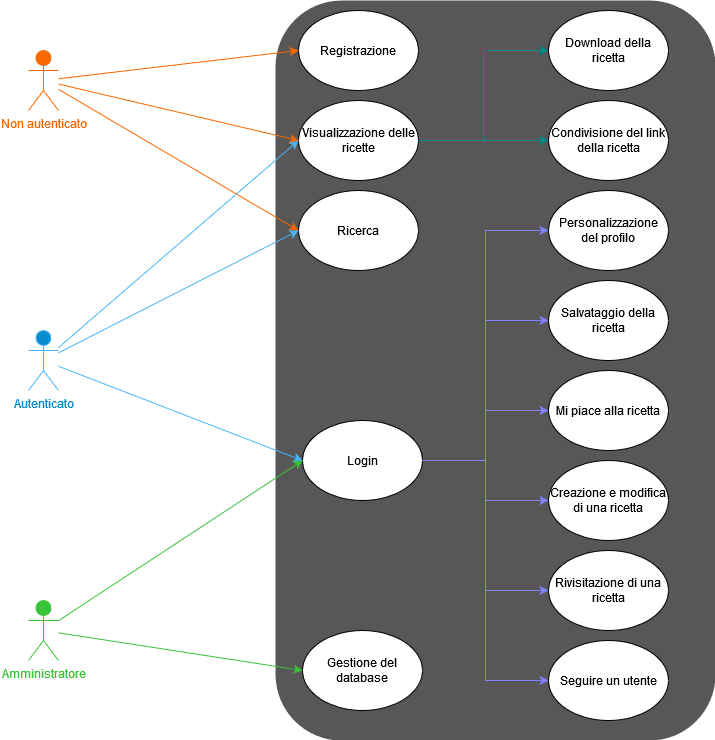
\includegraphics[width=1\textwidth]{./pictures/diagramma_operazioni.png}
                \caption{Diagramma delle operazioni}
                \label{fig:diagramma_operazioni}
            \end{figure}
    
    
    \newpage
    \section{Tecnologie usate}
        L'applicazione è sviluppata usando \href{https://www.djangoproject.com/}{\textbf{Django}} 
        sia lato backend che lato frontend.
        Il frontend fa uso del \textbf{Django Template Language (DTL)}, dell'\textbf{HTML}, 
        del \textbf{CSS} e del \textbf{JavaScript}; queste tecnologie permettono di 
        creare un interfaccia solida, dinamica e responsiva.
        Il backend fa uso principalmente di \href{https://www.python.org/}{\textbf{Python}} e \textbf{Javascript}.
        
        Sono state utilizzate anche delle librerie, in aggiunta, per semplificare e 
        migliorare alcuni aspetti dello sviluppo.
        
        Per l'interfaccia grafica è stata utilizzata la libreria \href{https://getbootstrap.com/}{\textbf{Bootstrap5}} 
        che permette di mantenere uno stile coerente per tutta l'applicazione; la maggior parte 
        delle icone, invece, sono state prese dalla libreria \href{https://fontawesome.com/}{\textbf{Font Awesome}} 
        mentre per i form sono staste utilizzate le app \textbf{crispy\_form} e \textbf{crispy\_bootstrap5}.
        
        Nel form per la creazione della ricetta è stata utilizzata l'app \\
        \textbf{django\_select2} che permette la ricerca degli ingredienti così 
        da velocizzarne la selezione.
        
        La maggior parte del codice scritto in javascript fa uso di \href{https://jquery.com/}{\textbf{jQuery}}; 
        inoltre per la modifica dinamica del contenuto degli elementi della pagina è stato utilizzato \textbf{Ajax}.
        
        La gestione dei dati è stata basata su \href{https://www.sqlite.org/}{\textbf{SQLite3}}, il database 
        predefinito in Django, veloce, leggero e ideale per l'utilizzo in locale.
        
        Per la converisone della pagina della ricetta in PDF è stata usata 
        \href{https://ekoopmans.github.io/html2pdf.js/}{\textbf{html2pdf}}.
        
        Per la ricerca si è fatto uso di \href{https://github.com/seatgeek/thefuzz}{\textbf{thefuzz}}
        e \href{https://github.com/rapidfuzz/RapidFuzz}{\textbf{rapidfuzz}} 
        le quali permettono un veloce confronto tra stringhe per un miglior risultato 
        e una migliore efficienza della ricerca.
        
        Le immagini delle ricette e dei profili sono gestite con \href{https://python-pillow.org/}{\textbf{Pillow}}
        la quale ha permesso di verificare, a tempo di caricamento, la validità dell'immagine, la dimensione 
        e il formato.
        
        Durante lo sviluppo è stata utilizzata \textbf{django-browser-reload} che ricarica 
        la pagina in automatico ad ogni modifica del codice eliminando il tempo di attesa 
        dal salvataggio del file alla ricarica manuale della pagina.
        
        In fine \textbf{django\_extensions} e \href{https://graphviz.org/}{\textbf{Graphviz}} 
        hanno permesso la creazione del diagramma UML dell'applicazione mentre \textbf{coverage} 
        ha permesso di calcolare la copertura dei test.
    
    
    \section{Organizzazione logica}
        Il programma è suddiviso in tre app ognuna delle quali gestisce un model e 
        delle view relative ad essi.
        
        \begin{itemize}
            \item \textbf{ingredient}: si occupa della registrazione e della modifica 
            degli ingredienti.
            
            \item \textbf{recipe}: gestisce la creazione e la modifica delle ricette;
            fornisce il form per la creazione, la pagina e la scheda delle ricette.
            
            \item \textbf{user}: è l'app relativa ai profili degli utenti; 
            fornisce la scheda, la pagina e metodi per la gestione e la creazione degli utenti.
        \end{itemize}
        
        La suddivisione del progetto in più app rende il codice più modulare e leggibile. 
        Ogni app ha un ambito di responsabilità ben definito, il che riduce la complessità 
        del progetto e ne facilita la manutenzione.
    
    
    \section{Scelte fatte}
        \subsection{Struttura delle pagine}
            Ho deciso di strutturare il sito in modo tale che non si verifichino caricamenti ogni 
            volta l'utente decide di spostarsi in un'altra sezione del sito, questo rende la navigazione 
            più fluida e piacevole per l'utente.
            Le uniche eccezioni sono quelle realtive alla pagina in cui viene visualizzata 
            la ricetta e la pagina personale degli altri utenti.
        
        
        \subsection{Recommendation system}
            Come sistema di raccomandazione ho scelto di utilizzare le interazioni dell'utente;
            nello specifico il model CustomUser memorizza un array di ingredienti che viene 
            aggiorato ogni volta che l'utente mette like o salva una ricetta, quindi viene 
            incrementato il valore di preferenza degli ingredienti relativi alla ricetta con cui
            l'utente ha interagito. Questo array viene utilizzato nella creazione della homepage 
            in cui vengono selezionate le ricette che potrebbero interessare all'utente.
        
        
        \subsection{Stile dell'applicazione}
            Ho scelto di usare bootstrap per mantenere uno stile coerente per tutta l'applicazione, 
            questo mi ha permesso di fornire un design uniforme e mi ha semplificato lo sviluppo dell'interfaccia grafica.
        
        
        \subsection{Scheda della ricetta}
            Nelle pagine iniziali dell'applicazione ho optato per la visualizzazione delle ricette 
            sottoforma di scheda, questo permette di avere un'antreprima della ricetta mostrando 
            un'immagine del piatto, il titolo e una breve descrizione.
            In questo modo l'utente può scegliere in se visualizzare la ricetta completa dopo averne avuto 
            un'anteprima.
        
        
        \subsection{Casricamento delle schede}
            Ogni pagina che mostra delle schede, possano essere delle ricette o degli utenti,
            utilizza il pagination system così da non riempire la pagina con troppi elementi ma 
            visualizzarne solo una parte.
            Ad ogni richiesta di una pagina del pagination system viene restituita una lista degli elementi
            che devono esere visualizzati, dopo di che uno script esegue in modo asincrono una richiesta per 
            ottenere la scheda relativa all'elemento da visualizzare; questo permette di caricare più elementi
            allo stesso tempo così da velocizzare il tempo di caricamento della pagina.
        
        
        \subsection{Critico gastronomico}
            Ogni utente può essere insignito del ruolo di critico gastronomico, questo 
            permette di elevare la probabilità con la quale una sua ricetta possa essere 
            mostrata nella pagina di un utente o durante una ricerca.
            Il ruolo aggiunge un icona accanto al nickname e può essere assegnato solo da un amministratore.
        
        
        \subsection{Remix}
            Un utente può scegliere di creare una nuova versione di una ricetta postata 
            da qualcun'altro, un remix della ricetta. Questo permette di conoscere l'utente che 
            ha scritto la ricetta originale, in oltre permette di consigliare le varianti della ricetta
            permettendo all'utente di trovare più facilmente la versione che preferisce.
    
    
    \section{Test}
        Sono stati eseguiti i test su la maggior parte del codice, nello specifico sulle 
        funzioni delle view, dei models e dei form.
        In totale i test coprono il 94\% del codice, questo dato è stato ottenuto tramite 
        il tool coverage che ha permesso di generare un report in HTML della copertura dei test;
        il report può essere visualizzato tramite il file \href{run:./../../applicazione/htmlcov/index.html}{index.html} 
        situato in \code{applicazione/htmlcov/}
    

    \section{Risultati}
        Il programma è completamente funzionante e offre tutte le funzionalità descritte.
        Ci sono alcuni margini di miglioramento, ad esempio la relazione tra i modelli 
        potrebbe essere migliorata e si potrebbero aggiungere alcune funzioni come la cancellazione
        del profilo o di una ricetta.

        Di seguito sono riportate alcune immagini dell'applicazione:
        \begin{figure}[ht]
            \centering
            \fbox{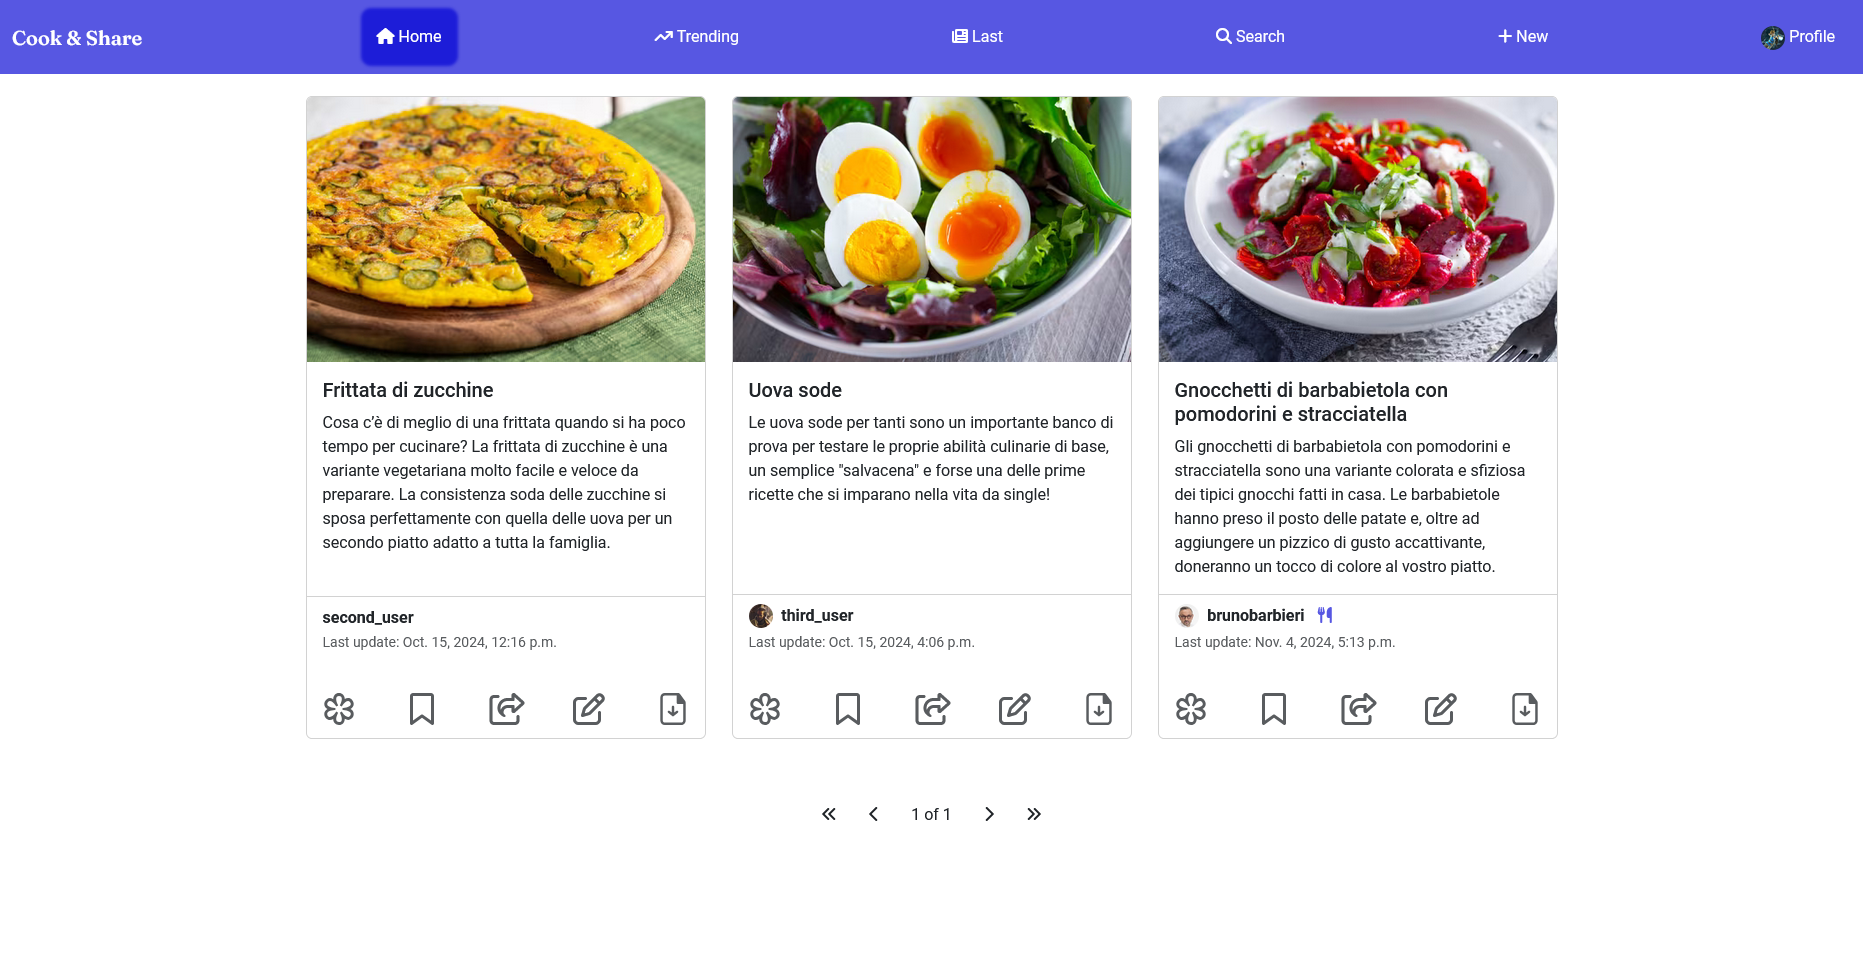
\includegraphics[width=.95\textwidth]{./pictures/homepage.png}}
            \caption{Homepage dell'applicazione}
            \label{fig:homepage}
        \end{figure}

        \begin{figure}[ht]
            \centering
            \fbox{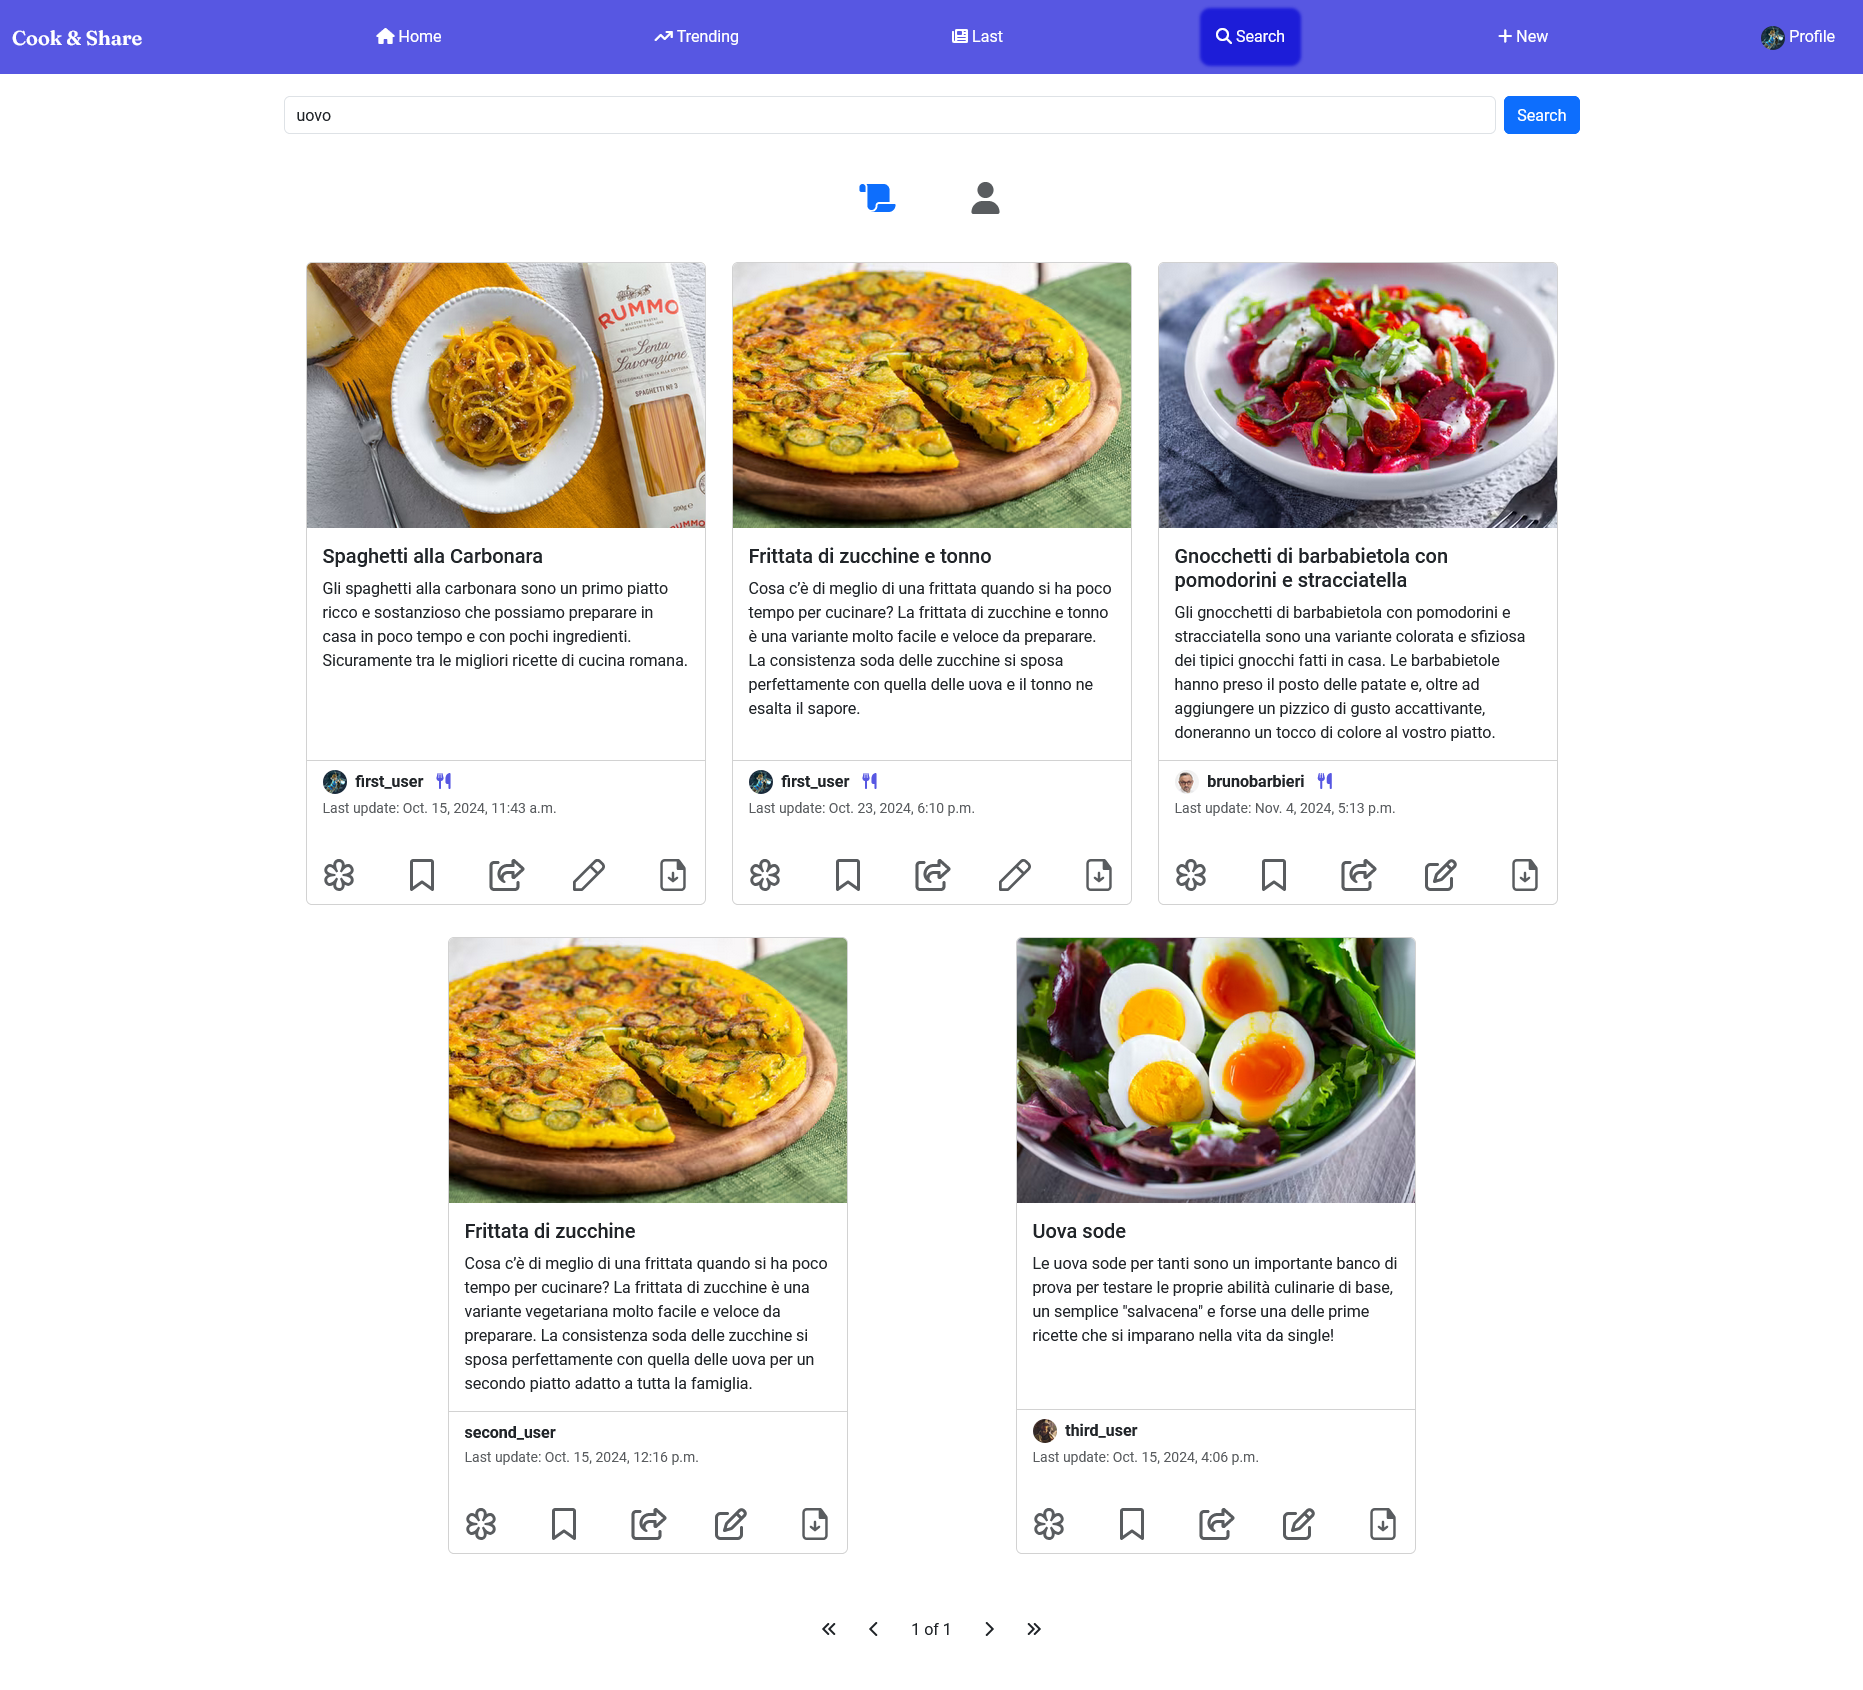
\includegraphics[width=.95\textwidth]{./pictures/search_recipe.png}}
            \caption{Ricerca delle ricette}
            \label{fig:search_recipe}
        \end{figure}

        \begin{figure}[ht]
            \centering
            \fbox{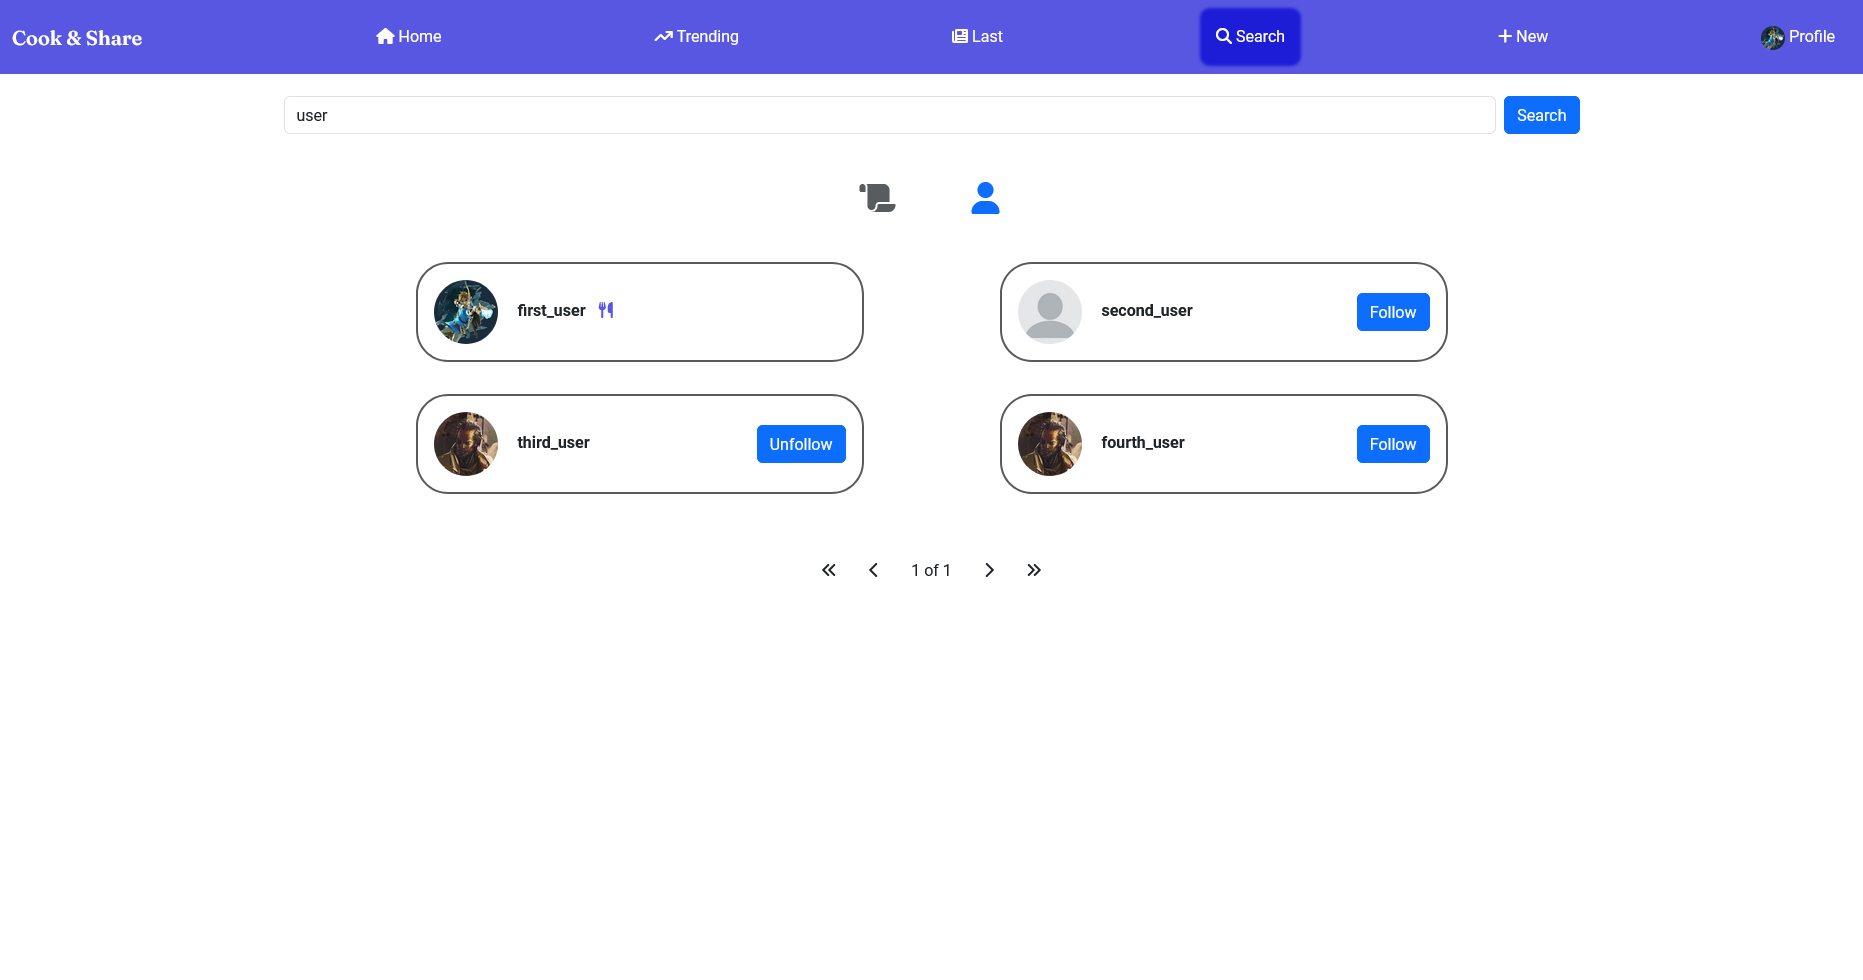
\includegraphics[width=.95\textwidth]{./pictures/search_user.png}}
            \caption{Ricerca degli utenti}
            \label{fig:search_user}
        \end{figure}

        \begin{figure}[ht]
            \centering
            \fbox{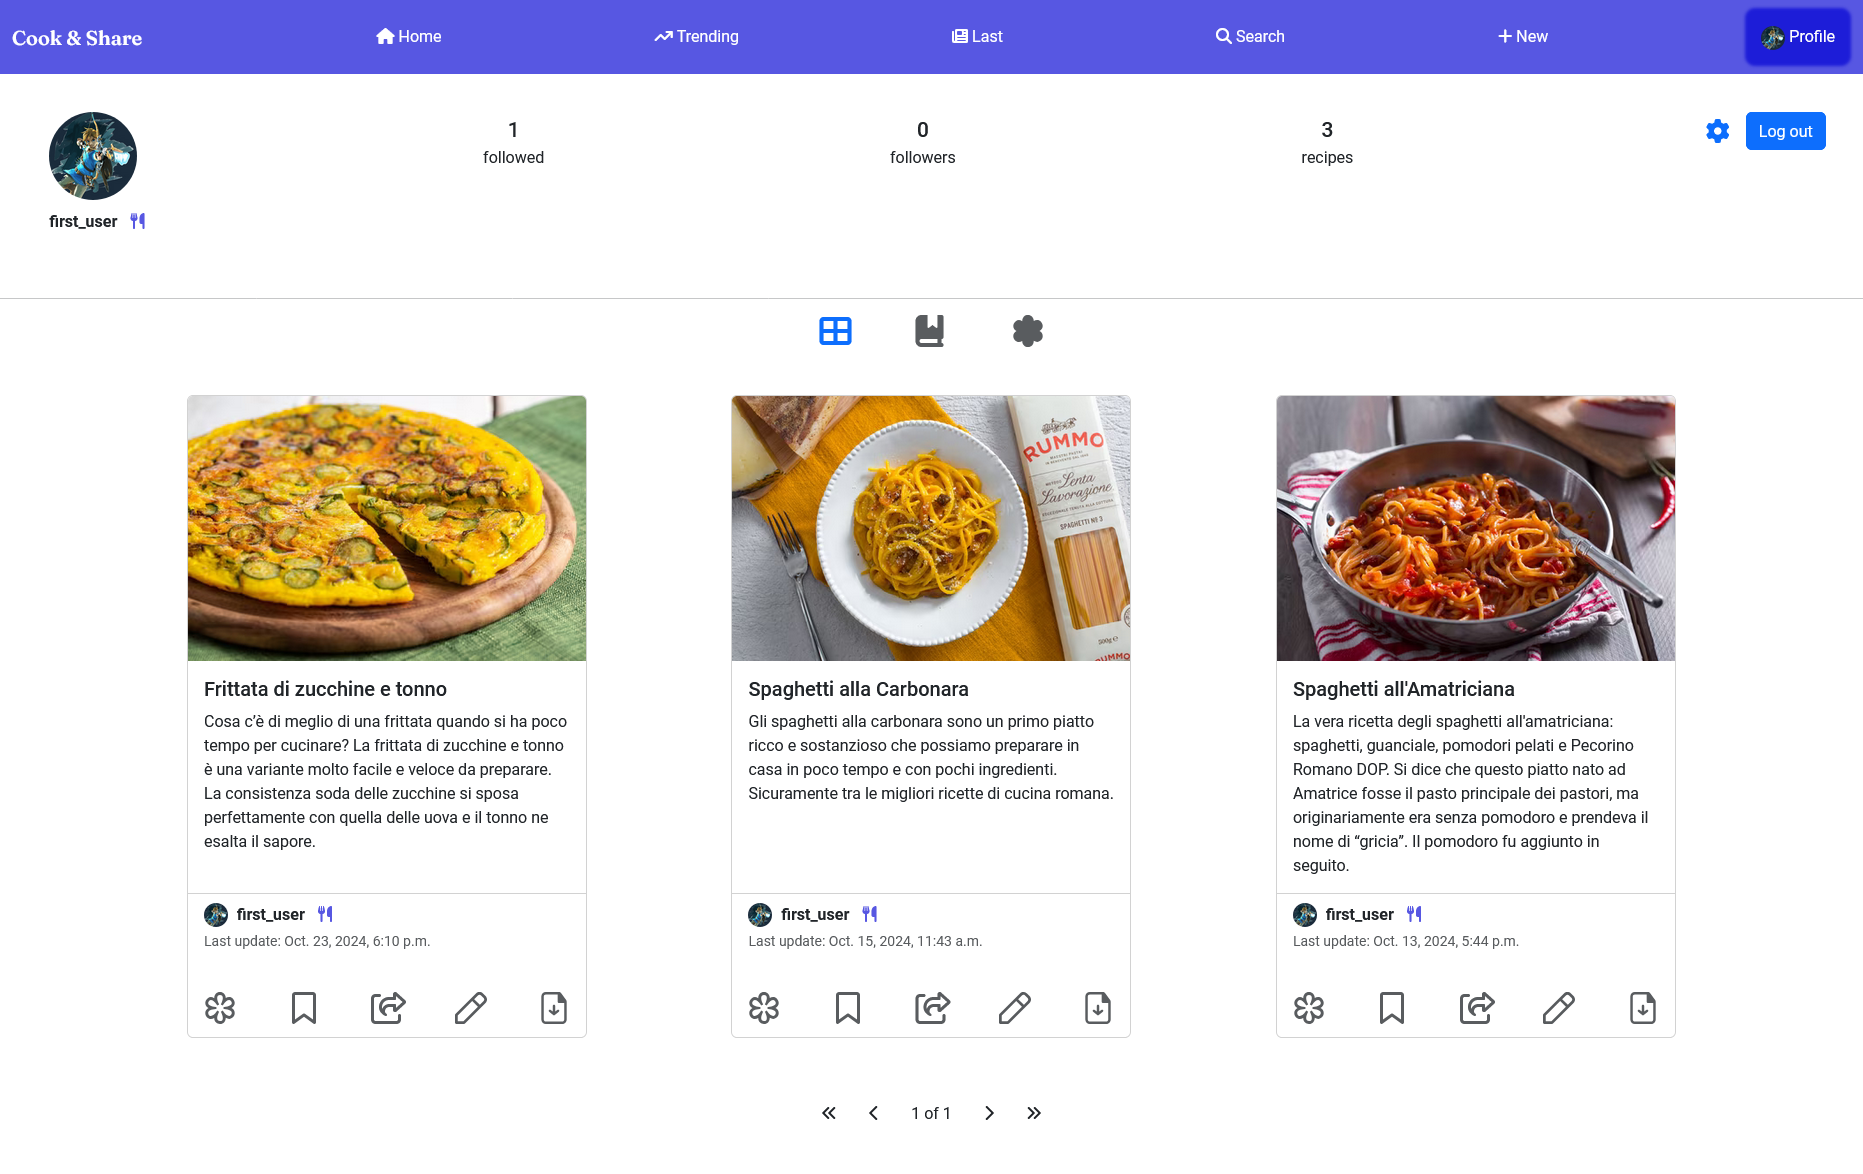
\includegraphics[width=.95\textwidth]{./pictures/profile_page.png}}
            \caption{Pagina dell'utente}
            \label{fig:profile_page}
        \end{figure}
        
        \begin{figure}[ht]
            \centering
            \fbox{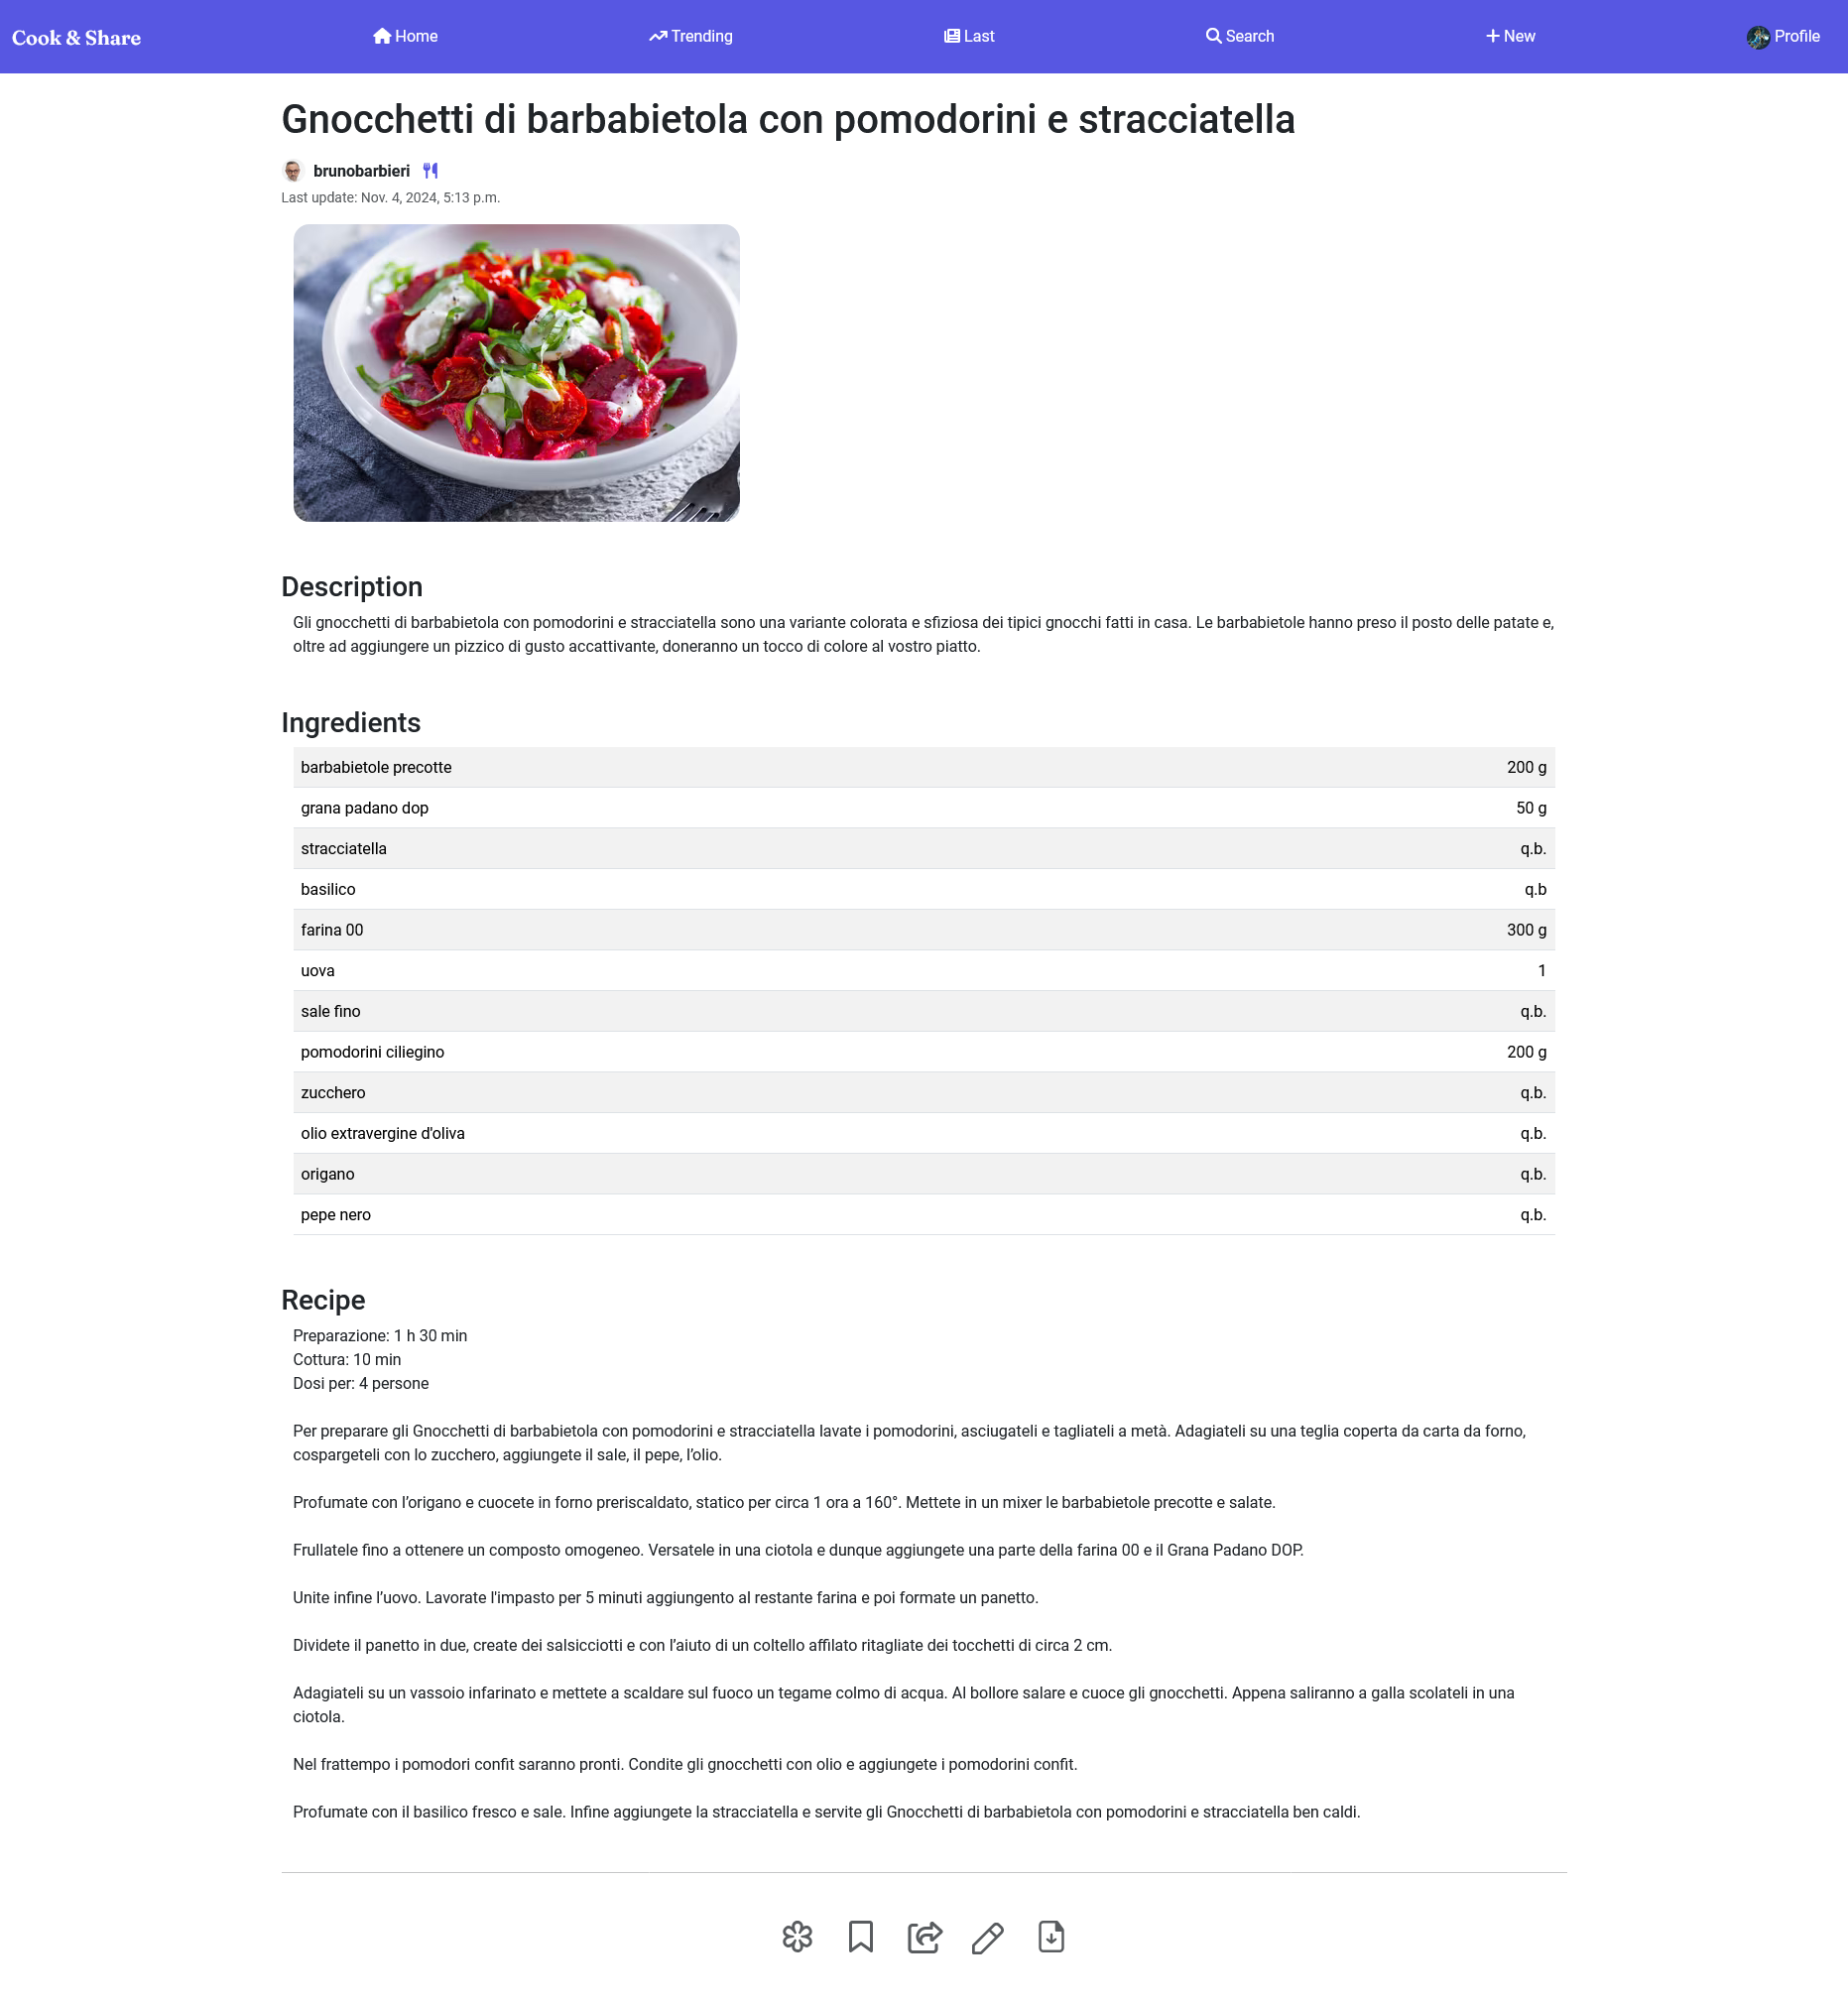
\includegraphics[width=.95\textwidth]{./pictures/recipe_page.png}}
            \caption{Pagina della ricetta}
            \label{fig:recipe_page}
        \end{figure}
\end{document}